\graphicspath{{./Wstep/images}}

\chapter{Wstęp}

Organizmy ziemskie ewoluowały w obecności pola grawitacyjnego. Na drodze ewolucji
 fizjologia tych organizmów jest nieustannie adaptowana do zewnętrznych bodźców, do których
  również należy zaliczyć siłę grawitacji. Oznacza to iż procesy sterujące wzrostem tych
   organizmów są optymalizowane względem środowiska z obecną siłą grawitacji. Rodzi to
    wiele pytań związanych z tym jak będzie przebiegał rozwój w środowiskach ze zredukowaną
     siłą grawitacji lub w stanie nieważkości. Badania nad tą materią są kluczowe dla
      odpowiedniego przygotowania się na przyszłe misje kosmiczne jak i mogą okazać się
       przydatne w zrozumieniu zasady działania owych procesów. Ten rozdział skupia się
        na różnych metodach badawczych studiowania organizmów i komórek w warunkach
         symulowanej mikrograwitacji oraz w szczegółach opisuje metodę bezpośrednio
          związaną z tematyką pracy - klinostatami. 

\section{Grawitropizm}

Grawitropizm jest nazwą zjawiska, które opisuje reakcję struktur wzrostowych na działającą
 na nie siłę grawitacji. W przypadku roślin zjawisko to odpowiada za rozwój systemu korzeni
  ku dołowi przy kiełkowaniu nasion oraz kieruje kierunkiem wzrostu pędów roślin ku górze
   \cite{bib:grawitropizm}. Taki mechanizm umożliwia roślinom dostosowanie swojej orientacji
   do otaczającego środowiska. Przeprowadzone badania wskazują iż w przypadku roślin, ważną
    rolę w percepcji sygnału grawitacyjnego odgrywają statocyty \cite{bib:statocyty}. Są to
     komórki ulokowane w  nasadce korzenia, w których dochodzi do sedymentacji gęstszych
      cząstek wypełnionych skrobią nazywanych statolitami \cite{bib:statocyty}. Ich ruch lub
       zmiana pozycji daje roślinie informacje o jej orientacji względem wektora grawitacji
        \cite{bib:statocyty}. Natomiast mechanizm jako całość nie jest jeszcze dobrze opisany
         \cite{bib:grawitropizm}.
        
     
\section{Symulatory mikrograwitacji}

Istnieje wiele sposobów imitacji środowiska kosmiczego w warunkach ziemskich. Część z
 rozwiązań jest uniwersalna względem testowanych obiektów, niektóre zaś są w stanie
  symulować owe warunki tylko dla wąskiego rodzaju obiektów badawczych. Poniżej opisane
   zostało kilka popularnych typów takich symulatorów.

\subsection{Lot paraboliczny}

Stan nieważkości w przypadku tego symulatora generowany jest przez lot samolotu po
 odpowiedniej trajektorii. Przystosowany do tego samolot wznosi się oraz spada pod kątem
  45$^\circ$. Gdy pojazd znajduje się na szczycie swojej trajektorii, cała zawartość
   samolotu doświadcza stanu nieważkości na czas około 20 sekund
    \cite{bib:lot_paraboliczny}. 

\begin{figure}[h]
	
	\centering
	
	
	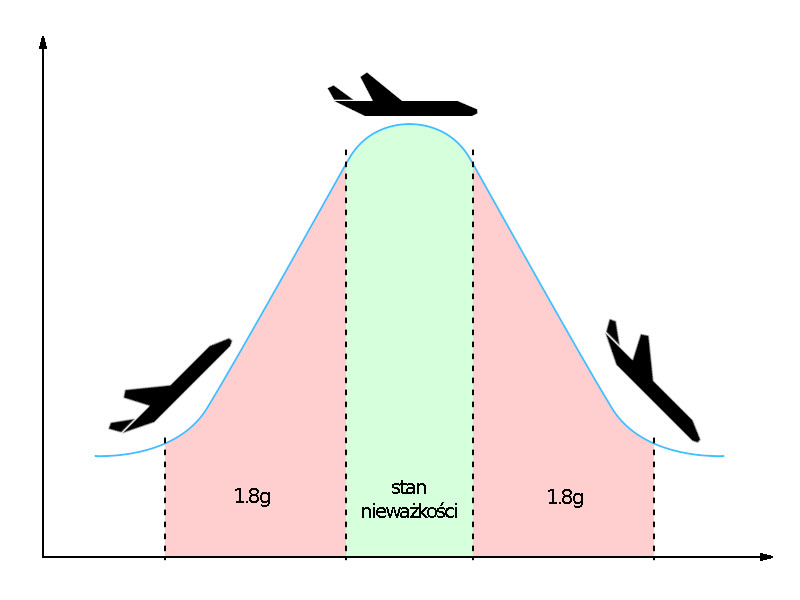
\includegraphics[scale=1.3]{lot_para_sch.jpg}
	\caption{Schemat trajektorii lotu parabolicznego.}
	\caption*{Źródło: opracowanie własne}
	\label{fig_paraboliczny}
	
\end{figure}

Metoda ta jest bardzo przydatna ze względu na możliwość poddania względnie dużych
 przedmiotów na warunki mikrograwitacji. Obecnie jest to jedyna metoda umożliwiająca
  wystawienie astronautów na takie warunki, przed wysłaniem ich na Międzynarodową Stację
   Kosmiczną (ISS)\cite{bib:lot_paraboliczny}. Samolot może również poruszać się po
    łuku, symulując w ten sposób środowisko o obniżonej, niezerowej grawitacji. Z tego
     typu symulatorów korzysta się również w początkowych etapach badań, przed decyzją o
      wysłanie obiektów badawczych w kosmos. Pozwala to zebrać użyteczne dane wstępne
       jak i zmodyfikować parametry eksperymentu docelowo przeprowadzanego w kosmosie.
        Wadą tego rozwiązania jest przede wszystkim krótki okres w którym ładunek
         doświadcza stanu nieważkości.

\subsection{Systemy LSMM}

\angver{Low-shear modeled microgravity} (LSMM) jest nazwą obejmującą szeroką gamę symulatorów używanych w przypadku próbek
 biologicznych. Ta grupa urządzeń symuluje pewne konkretne cechy środowiska kosmicznego
  takie jak brak sedymentacji cząstek, niskie naprężenia ścinające w płynach oraz niewielkie
   turbulencje \cite{bib:lsmm1}. Zwykle urządzenia tego typu wykorzystują rotację całej
    próbki aby osiągnąć wspomniane wcześniej cechy środowiska. Pierwsze bioreaktory
     rozwijane były przez Centrum Lotów Kosmicznych im. Lyndona B. Johnsona
       \cite{bib:lsmm1}, które służyły do badania rozwoju mikroorganizmów w warunkach
       mikrograwitacji. Tego typu urządzenia są zwykle kategoryzowane jako  \angver{Rotating Wall Vessel} (RWV), które
        następnie obejmuje wiele różnych konfiguracji takich jak \angver{High Aspect Ratio Vessel} (HARV), \angver{Slow Turning Lateral Vessel} (STLV), \angver{Rotating Wall Perfusion Vessel} (RWPV). W
         celach badań roślin, ludzkich komórek lub tkanek wykorzystuje się urządzenia
          nazywane klinostatami, które również należą do grupy systemów
           LSMM \cite{bib:nasa_space_biology} natomiast znacznie różnią się konstrukcją.
            Wariacją klinostatów są maszyny RPM. Tematyka tej pracy jest ściśle związana
             z klinostatami, a więc zostaną one omówione szczegółowo w dalszej częsci
              tego rozdziału.

\subsection{Lewitacja diamagnetyczna}

Kolejną metodą wykluczenia skutków oddziaływania siły grawitacji z próbką jest
 wykorzystanie interakcji diamagnetycznej. Diamagnetyzm jest fundamentalną cechą
  materii, powodowaną ruchem elektronów w atomach \cite{bib:kittel}. Zjawisko to można
   wykorzystać do lewitacji każdej substancji, wymagane jest jedynie odpowiednio silne
    zewnętrzne pole magnetyczne. Z uwagi na to iż diamagnetyzm jest oddziaływaniem
     bardzo słabym, stosowane są pola magnetyczne o indukcji rzędu \SI{16.5}{T}. Należy
      zaznaczyć iż aby osiągnąć stan lewitacji konieczne jest uzyskanie wysokiego
       przestrzennego gradientu pola magnetycznego, pole jednorodne nie będzie skutkować
        pojawieniem się sił związanych z diamagnetyzmem. Tego typu lewitacja została
         wykorzystana w badaniach nad rozwojem oraz ekspresją genów w muszkach owocowych
          (\angver{Drosophila melanogaster}) w warunkach
           mikrograwitacji \cite{bib:lewitacja}.

\subsection{Maszyny spadku swobodnego}

Pierwsze maszyny spadku swobodnego (ang. \angver{Free Fall Machine}, FFM) zostały wynalezione jako alternatywa dla już wtedy
 istniejących klinostatów dwuwymiarowych. Zasada działania tych urządzeń opiera się na
  grawitacyjnym spadku swobodnym próbki przymocowanej do wózka ślizgającego się wzdłuż
   pionowych szyn o długości \SI{1}{m} \cite{bib:ffm_rpm}. Gdy próbka opada na dół
    urządzenia, podmuch sprężonego powietrza o ciśnieniu \SI{8}{bar} odbija próbkę z
     powrotem na górę szyny i cykl się powtarza. Istnieje minimalny próg czasowy
      rejestracji zmian grawitacji dla próbek biologicznych \cite{bib:ffm}. Jeśli okres
       doświadczania wysokiego przeciążenia podczas powrotu próbki na górę urządzenia
        jest wystarczająco krótki, to rejestrowane są jedynie momenty spadku swobodnego.
         W ten sposób całość stymulacji odbierana jest jako długotrwały okres
          mikrograwitacji \cite{bib:ffm}.

\section{Klinostaty} \label{klinostaty}

Jak wspomniano w poprzednim podrozdziale, klinostaty są urządzeniami z grupy systemów
 LSMM, co oznacza, że ich celem jest imitacja pewnych cech środowiska mikrograwitacji
  dla próbek biologicznych. Podobnie jak maszyny FFM wykorzystują one minimalny czas
   odpowiedzi układu biologicznego na stymulację
    grawitacyjną \cite{bib:klinostat_lafayette}. Ciągłe zmiany wektora grawitacji
     względem badanej próbki zapobiegają kierunkowej odpowiedzi
      układu \cite{bib:klinostat_lafayette}. Ta sama zasada może również zostać
       wykorzystana w celu symulacji mniejszego przyspieszenia grawitacyjnego niż
        ziemskie np. księżycowego lub marsjańskiego. Jakość wytworzonego symulowanego
         stanu mikrograwitacji zależy od wielu czynników, takich jak: czas odpowiedzi
          układu na stymulację czy temperatura \cite{bib:klinostat_lafayette}.
           Konstrukcje podobne do klinostatów mogą zostać również wykorzystane w
            symulacjach środowiska hipergrawitacyjnego poprzez wykorzystanie siły
             odśrodkowej. Kluczowe jest zrozumienie iż klinostaty nie odtwarzają stanu
              mikrograwitacji, a jedynie kompensują skutki działania grawitacji na
               systemy biologiczne. Niemniej w ramach uproszczenia, w dalszej części
                pracy, stan ten będzie nazywany mikrograwitacją.
                


\section{Zasada działania klinostatu}

Klinostaty w celu wytworzenia stanu mikrograwitacji wykorzystują ruch obrtotowy, badź
 złożenie dwóch ruchów obrotowych o osiach prostopadłych względem siebie. Próbka
  znajdująca się na platformie wewnątrz klinostatu doświadcza zmieniającego się w czasie
   wektora grawitacji, z uwagi na to, iż zmienia się jej orientacja względem ów wektora.
    Obroty te dobrane są tak aby działanie wektora grawitacji zostało uśrednione w
     czasie, dając w rezultacie brak oddziaływania. Mogą być one stałe w czasie i zgodne
      w kierunku (dotyczy klinostatów 2-D oraz 3-D), lub całkowicie niezależne od siebie
       (maszyny RPM). Szybkość zadanych obrotów zależy od parametrów wspomnianych w
        podrozdziale \ref{klinostaty}. Dla roślin czas reakcji układu wynosi około 1 do
         2 min. \cite{bib:klinostat_lafayette}. W związku z tym klinostaty w celach badań
          nad roślinami zwykle obracają się z prędkościami 1 do 2 RPM. Klinostaty do
           badań mikroorganizmów wymagają znacznie większych prędkości obrotowych aby
            zapewnić kompensajcę sedymentacji zawiesin.
            

\section{Rodzaje klinostatów}

Wyróżnia się trzy główne typy klinostatów, dzielone ze względu na liczbę stopni swobody
 oraz rodzaj obrotów dostępnych osi. Rodzaje te zostały wspomniane w podrozdziałach
  poprzednich, a poniżej znajduje się ich krótkie rozwinięcie.

\subsection{Klinostat 2-D}

Klinostat o tylko jednej osi obrotu. Oś ta może być zorientowana na dwa sposoby -
 prostopadle do wektora grawitacji i osi korzenia (klinorotacja wertykalna) lub
  prostopadle do wektora grawitacji i równolegle do osi korzenia (klinorotacja
   horyzontalna) \cite{bib:klinorotacja} . Ilustracja rodzajów klinorotacji
    przedstawiona jest na Rys. \ref{fig:klinorotacje}. Próbka zamocowana na
     obracającej się platformie doświadcza uśredniania ów wektora tylko w jednym
      kierunku. Jest to najwcześniejszy typ klinostatów oraz jest najprostszy w
       konstrukcji. Klinostat ten nazywany jest klinostatem dwuwymiarowym (2-D) ze
        względu na zmianę orientacji próbki względem wektora grawitacji tylko w jednej
         płaszczyźnie.

\begin{figure}
	
	\centering
		\begin{subfigure}[b]{.49\textwidth}
		\centering
		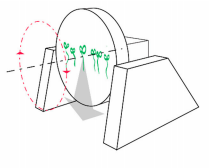
\includegraphics[width=.7\textwidth]{klinorot_wert}
		\caption{Klinorotacja wertykalna.} 
		\label{fig:klinorot_wert}
	\end{subfigure}
	\hfill%
	\begin{subfigure}[b]{.49\textwidth}
		\centering
		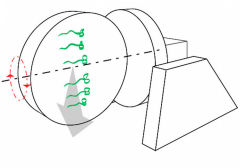
\includegraphics[width=.7\textwidth]{klinorot_hor}
		\caption{Klinorotacja horyzontalna.} 
		\label{fig:klinorot_hor}
	\end{subfigure}

	\caption{Rodzaje klinorotacji 2-D. Źródło: \cite{bib:klinorotacja}} 
	\label{fig:klinorotacje}
	
\end{figure}

\subsection{Klinostat 3-D} \label{klinostat3d}

Klinostat trójwymiarowy ma jedną dodatkową oś obrotu względem klinostatu dwuwymiarowego.
 Typowy klinostat 3-D składa się z zewnętrznej ramy, stanowiącej pierwszy stopień
  swobody, która obraca się wokół własnej osi symetrii. Wewnątrz ramy znajduje się
   kolejny stopień swobody zwykle w postaci już miejsca zamocowania badanego obiektu,
    który ma możliwość obrotów wokół osi prostopadłej do osi obrotu ramy zewnętrznej.
     Nie jest to natomiast jedyny sposób konstrukcji tego urządzenia. Wewnętrzne stopnie
      swobody klinostatów 3-D znacznie różnią się pomiędzy gotowymi urządzeniami, ze
       względu na to iż często są dopasowywane do docelowych obiektów badań. W typowym
        dwuwymiarowym klinostacie oba stopnie swobody obracają się w tym samym kierunku,
         ze stałą prędkością. W niektórych sytuacjach może to powodować niesymetryczne
          pokrycie dostępnych kierunków przestrzennych \cite{bib:rpmy}, co nie jest
           porządane. Rozwiązaniem tego problemu jest wprowadzenie losowości do ruchu
            obydwu stopni swobody poprzez zmianę prędkości oraz kierunku obrotów w
             czasie \cite{bib:rpmy}. Urządzenia realizujące tego typu strategię nazywamy
              maszynami losowego pozycjonowania (RPM). Charakteryzuje je lepsze pokrycie
               wszystkich kierunków przestrzennych. Maszyny RPM mogą pracować w trybach
                odpowiadających każdemu z trzech rodzajów klinostatów. Przykładowa
                 maszyna RPM przedstawiona została na Rys. \ref{fig_rpm}.

\begin{figure}
	\centering
	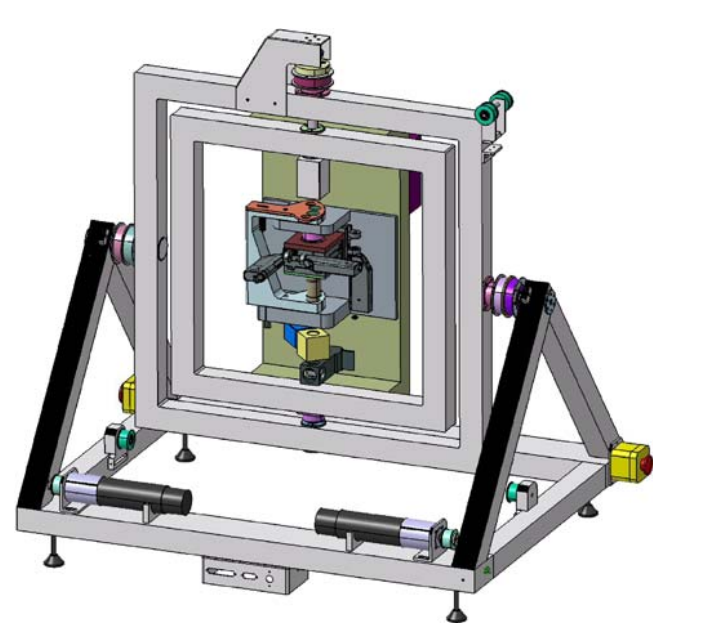
\includegraphics[scale=0.5]{rpm}
	\caption{Przykładowa maszyna RPM, zawierająca mikroskop fluorescencyjny} 
	\caption*{Źródło: \cite{bib:rpmy}}
	\label{fig_rpm}
\end{figure}

\section{Obecne rozwiązania}

Znaczna część badań korzystająca z klinostatów przeprowadzana jest w urządzeniach
 wykonanych specjalnie na ich potrzebę. Niemniej istnieją otwartoźródłowe projekty urządzeń
  tego typu oraz szereg rozwiązań dostępnych komercyjnie. Z uwagi na niszowość tego sektora
   urządzenia dostępne na rynku są drogie. Przykładowo koszt maszyny RPM firmy Yuri Gravity
    o wymiarach platformy 15x15x15 cm wynosi \SI{45900}{\geneuro}, wraz z komputerem oraz oprogramowaniem. Duża część rozwiązań dostępnych na rynku skupia
     się wokół badań nad mikroorganizmami, co powoduje, że konstrukcja tych urządzeń
      uniemożliwia badania nad innymi typami ogranizmów np. roślinami. W związku z tym, jeśli
       zachodzi konieczność użycia maszyny RPM lub klinostatu 3-D w badaniach nad
        organizmami roślinnymi, częstym rozwiązaniem jest projekt urządzenia dostosowany do
         indywidualnych potrzeb. Taki projekt klinostatu zrealizowano w ramach projektu PBL w którym
          uczestniczyłem dwa lata temu i to niemu poświęcony jest kolejny rozdział.
          
